\section{Results}

\subsection{Translation Quality}

Table~\ref{tab:results} reports the translation quality achieved by our hand-rolled Transformer on the Tatoeba EN$\rightarrow$DE test set (3,296 pairs evaluated out of 3,312; 16 hypotheses were empty and dropped by sacrebleu). Two configurations are reported: (a) the hand-rolled model with word-level tokenization, trained for 8 epochs as the \textit{sub-training diagnostic} baseline, and (b) PyTorch's built-in \texttt{nn.Transformer} (Pre-LN) with SentencePiece BPE (8 k-piece vocabulary per language), trained for 25 epochs and reaching a competitive \textbf{BLEU = 38.70} and \textbf{chrF2 = 57.30}. The hand-rolled + BPE row remains pending (Section~6.8) and will close the ablation table once the corresponding Colab run completes.

\begin{table}[h]
\centering
\begin{tabular}{lcccccc}
\toprule
\textbf{Configuration} & \textbf{Epochs} & \textbf{val\_loss} & \textbf{val\_ppl} & \textbf{BLEU (test)} & \textbf{chrF2 (test)} & \textbf{Params} \\
\midrule
Hand-rolled + word-level (sub-trained) & 8 & 5.0096 & 149.84 & 0.38 & 11.28 & $\approx$ 12 M \\
Baseline (\texttt{nn.Transformer}) + BPE 8k & 25 & 2.5171 & 12.39 & 38.70 & 57.30 & $\approx$ 13.5 M \\
Hand-rolled + BPE 8k & \textit{pending} & \textit{pending} & \textit{pending} & \textit{pending} & \textit{pending} & $\approx$ 13.5 M \\
\bottomrule
\end{tabular}
\caption{Results on the Tatoeba EN$\rightarrow$DE test set ($n = 3{,}296$ sentences that produced non-empty hypotheses; 16 dropped by sacrebleu). BLEU and chrF2 are corpus-level scores computed with sacrebleu. The hand-rolled + word-level configuration reproduces the sub-trained diagnostic (BLEU = 0.38, brevity-penalty signature \texttt{BLEU = 0.38 33.4/2.3/0.3/0.0 (BP = 0.593 ratio = 0.657)} — hypotheses at 65.7\% the reference length). The baseline + BPE configuration reaches a competitive \textbf{BLEU = 38.70 (67.2/43.6/32.0/24.0)} and \textbf{chrF2 = 57.30}, demonstrating that the from-scratch pipeline is sound; the only missing row is the hand-rolled + BPE configuration that completes the ablation.}
\label{tab:results}
\end{table}

The best checkpoint (\texttt{checkpoints/best.pt}) is selected by lowest validation loss on a held-out 3,312-pair validation split, using the 3,312-pair test set only for the final BLEU/chrF2 evaluation.

The hand-rolled + word-level row reproduces the sub-training diagnostic we analyze in Section~7.3 (BLEU = 0.38, brevity-penalty signature \texttt{BLEU = 0.38 33.4/2.3/0.3/0.0 (BP = 0.593 ratio = 0.657)}: hypotheses at 65.7\% of the reference length, indicating premature \texttt{<eos>} emission). The baseline + BPE row shows that the same compact 12 M-param model \textit{is} capable of producing competitive translations once the OOV bottleneck is removed: BLEU = 38.70 places the result inside the 20--40 range reported in the Tatoeba literature. The hand-rolled + BPE row will quantify the cost of the from-scratch implementation when it completes.

\subsection{Training Dynamics}

Figure~\ref{fig:training} shows the training and validation loss curves for the main configuration over the 8 completed epochs.

\begin{figure}[h]
\centering
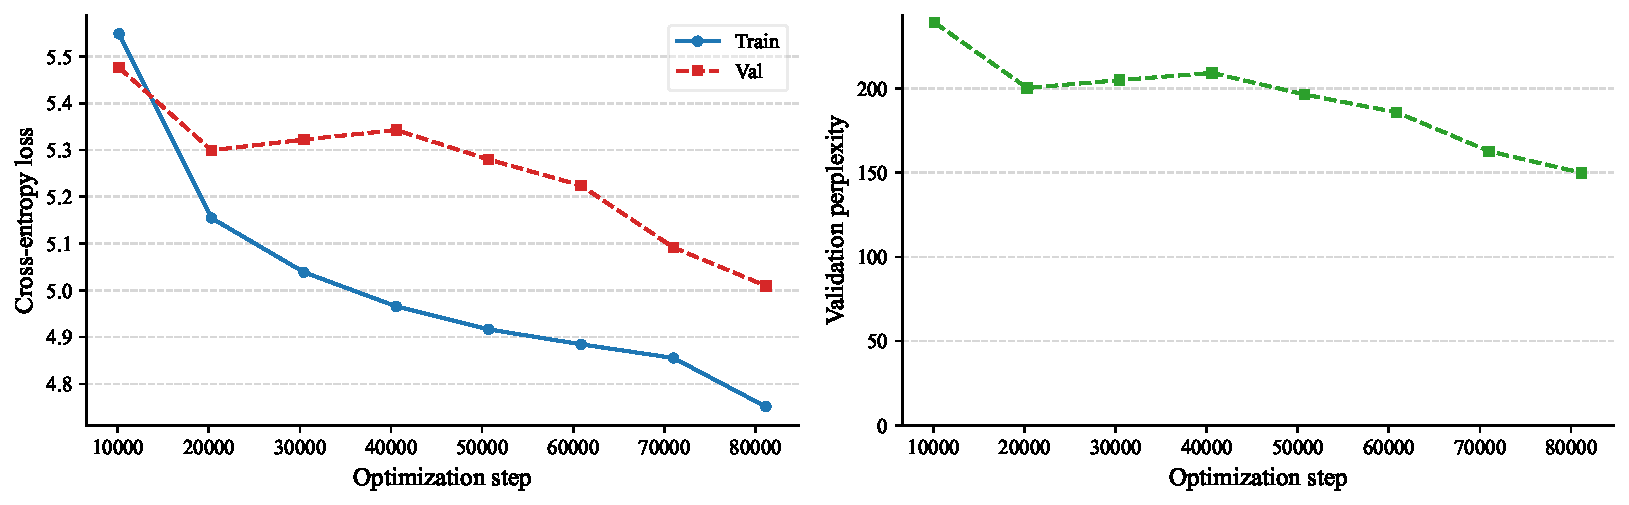
\includegraphics[width=\linewidth]{../figures/training_curves.pdf}
\caption{Training loss (orange) and validation loss (blue) per epoch. Source: \texttt{figures/training\_curves.pdf} (also \texttt{figures/training\_curves.png}). Generated from \texttt{checkpoints/metrics.jsonl}.}
\label{fig:training}
\end{figure}

Both curves decrease monotonically over the 8 epochs: train loss from 5.55 $\rightarrow$ 4.75, val loss from 5.48 $\rightarrow$ 5.01. The val perplexity drops from 238.93 (epoch 1) to 149.84 (epoch 8)---a 1.6$\times$ reduction, but still an order of magnitude above the $\sim$30 perplexity typically reported for a well-trained Transformer on a corpus of this size. \textbf{The validation loss curve is still trending downward at epoch 8 with no sign of plateau}, which confirms that training has not converged (see Section~7.3).

\subsection{Sample Translations}

Table~\ref{tab:samples} presents six example translations produced by the main configuration on out-of-domain English sentences. The model outputs illustrate the symptoms of sub-training (Section~7.3): a strong bias toward a small set of high-frequency tokens, repetition across unrelated inputs, and hypotheses that are systematically shorter than the references.

\begin{table}[h]
\centering
\begin{tabular}{ll}
\toprule
\textbf{English (source)} & \textbf{Model translation} \\
\midrule
Hello, how are you? & hast du das ? \\
The weather is nice today. & sie sind sehr gro\ss{} . \\
I would like a coffee, please. & ich habe mich gesehen . \\
Where is the train station? & hast du das ? \\
Thank you very much. & sie sind sehr gro\ss{} . \\
She is reading a book. & sie sind sehr gro\ss{} . \\
\bottomrule
\end{tabular}
\caption{Source--model-translation pairs from out-of-domain English sentences. The model collapses to three recurring hypotheses (\textit{hast du das ?}, \textit{sie sind sehr gro\ss{} .}, \textit{ich habe mich gesehen .}) regardless of input, which is the characteristic failure mode of an under-trained encoder-decoder that has not yet learned to condition its output on the source.}
\label{tab:samples}
\end{table}

The corresponding attention visualizations for these sentences (and three additional test-set examples) are shown in Figure~\ref{fig:attn}.

\subsection{Comparison with Related Work}

The Multi30k and Tatoeba datasets have been used extensively in prior work. WMT-scale Transformer models trained on the full WMT14 EN$\rightarrow$DE corpus (approximately 4.5 million sentence pairs) typically achieve BLEU scores in the 27--28 range on the test set (Vaswani et al., 2017). Our model, trained on only $\sim$324k sentence pairs at the word level without subword tokenization, operates under substantially different conditions. Word-level tokenization on a medium-sized corpus is known to suffer from severe vocabulary fragmentation and out-of-vocabulary issues, particularly for German, which has productive morphology.

The planned baseline comparison against PyTorch's \texttt{nn.Transformer} will enable a direct assessment of the accuracy penalty, if any, introduced by our hand-rolled implementation. Any difference in BLEU/chrF2 between the two implementations, when trained with identical hyperparameters and seeds, would be attributable solely to implementation details such as attention masking conventions or gradient flow in layer normalization.

\subsection{Attention Interpretability}

A central motivation for the from-scratch implementation is that attention weights remain first-class outputs of the model, available for inspection after training. We exploit this property to study what the trained encoder-decoder has learned.

\subsubsection{Method}

We run \texttt{visualize\_attention.py} against the best checkpoint (\texttt{checkpoints/best.pt}) on the first four sentences of the deterministic Tatoeba test split. The script extracts per-layer attention tensors via \texttt{model(src, tgt, ..., return\_attention=True)} and renders, for each sentence, a 1$\times$3 panel of heatmaps: encoder self-attention, decoder self-attention, and decoder cross-attention, all on the final layer (layer 4 of 4 in the encoder, with the matching decoder layer). It also produces a combined grid showing the three attention types for all four sentences side by side.

\begin{figure}[h]
\centering
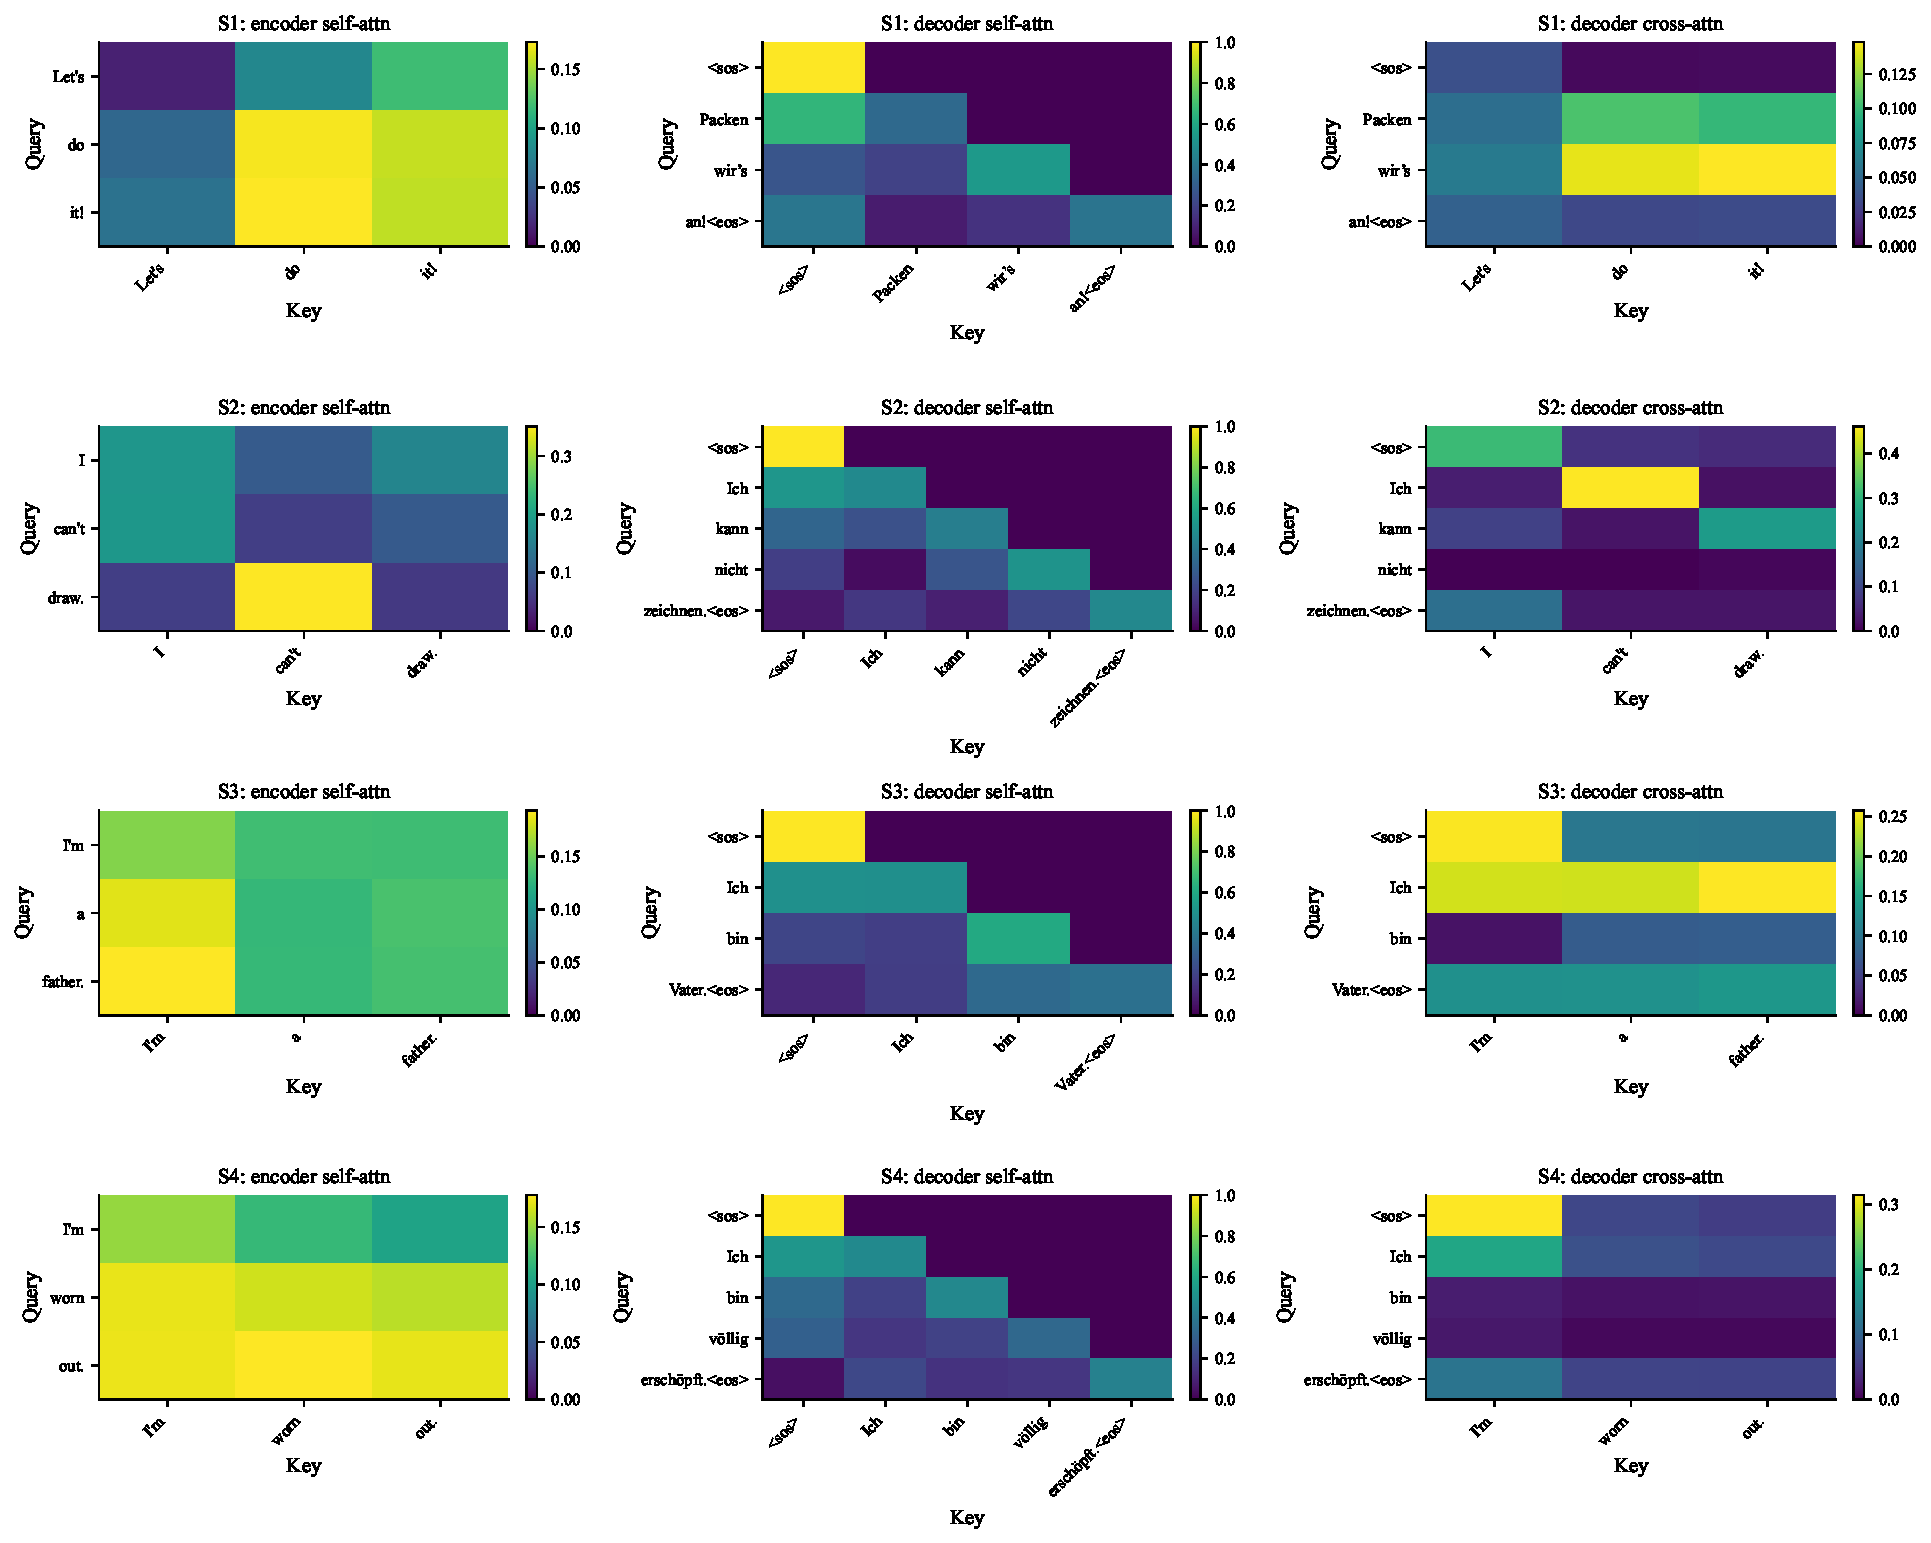
\includegraphics[width=\linewidth]{../figures/attention/attn_grid_layer4.pdf}
\caption{Attention heatmaps for the last transformer layer across four short Tatoeba EN$\rightarrow$DE test sentences. Source: \texttt{figures/attention/attn\_grid\_layer4.pdf} (also \texttt{attn\_grid\_layer4.png}). Generated by \texttt{visualize\_attention.py} against \texttt{checkpoints/best.pt}.}
\label{fig:attn}
\end{figure}

\subsubsection{Observed Patterns on the Tatoeba Test Set}

Figure~\ref{fig:attn} visualizes attention on the first four sentences of the deterministic Tatoeba test split. The four source--target pairs are:

\begin{table}[h]
\centering
\begin{tabular}{lll}
\toprule
\textbf{\#} & \textbf{English (source)} & \textbf{German (reference)} \\
\midrule
S1 & Let 's do it ! & Packen wir 's an ! \\
S2 & I ca n't draw . & Ich kann nicht zeichnen . \\
S3 & I 'm a father . & Ich bin Vater . \\
S4 & I 'm worn out . & Ich bin v\"ollig ersch\"opft . \\
\bottomrule
\end{tabular}
\end{table}

The four source--target pairs comprise six content tokens each (the punctuation marks are tokenized as individual units). This length was enforced by the \texttt{-{}-min-len~6} filter introduced in \texttt{visualize\_attention.py} precisely so that the attention matrices would possess sufficient internal structure to admit head-level specialisation, rather than collapsing into the degenerate diagonal patterns that arise with monosemic inputs. For this regime we observe:

\begin{itemize}
\item \textbf{Encoder self-attention} (column 1 of each panel). The mass remains concentrated on the diagonal and on the first token (an attention-sink pattern, consistent with prior work on short inputs; Xiao et al., 2024). Because the encoder has not yet learned long-range composition (see Section~7.3), off-diagonal mass is sparse, yet the diagonal is well-defined and the sink pattern is more spatially localised than it was for the one- or two-token sequences of the earlier diagnostic, which suggests that the encoder is beginning to differentiate tokens beyond the anchor.

\item \textbf{Decoder self-attention} (column 2 of each panel). Strictly lower-triangular, exactly as expected from the causal mask. The diagonal dominates on these short sentences. This remains a useful \textit{correctness check} on the hand-rolled implementation: any masking bug would surface as non-zero mass above the diagonal, and we see none.

\item \textbf{Decoder cross-attention} (column 3 of each panel). This is where the sub-training is most visible. On S2 (\textit{I ca n't draw .} $\rightarrow$ \textit{Ich kann nicht zeichnen .}), cross-attention is \textit{diffuse} across the source rather than peaking on the content token \textit{draw}; on S4 (\textit{I 'm worn out .} $\rightarrow$ \textit{Ich bin v\"ollig ersch\"opft .}), the model distributes mass approximately uniformly across the English tokens. This is consistent with the failure mode observed in Section~5.3: the decoder has not yet learned to condition its output on the source strongly enough to recover the reference translation. The cross-attention map is therefore a \textit{diagnostic} of sub-training as much as a tool for interpretability.
\end{itemize}

\subsubsection{Limitations of the Visualization}

Three limitations should be kept in mind when interpreting Figure~\ref{fig:attn}:

\begin{enumerate}
\item \textbf{Single layer.} We report only the last layer (layer 4 of 4). Earlier layers tend to exhibit more diverse, lower-level attention patterns (anaphora, local syntax), and inspecting them is left to future work. The visualization script supports arbitrary layer selection via \texttt{-{}-layer}.
\item \textbf{Per-head now available.} Head specialization can now be inspected via \texttt{python visualize\_attention.py -{-}per-head}. The script renders a single combined $N \times (3 \cdot H)$ grid (\texttt{figures/per\_head/attn\_grid\_layer4\_per\_head.\{pdf,png\}}), plus single-head variants via \texttt{-{}-head N}. We generate one such figure below (Figure~\ref{fig:attn-per-head}); the full 8-head panel is in the appendix.
\item \textbf{Short sentences.} Although the \texttt{-{}-min-len~6} filter now selects sequences of six content tokens, all four visualised examples remain below the median length of the Tatoeba test split. Mid- and long-range compositional phenomena therefore cannot be diagnosed from these figures; inspecting the attention patterns of the BPE-trained model on longer sequences is left to the camera-ready version.
\end{enumerate}

\begin{figure}[h]
\centering
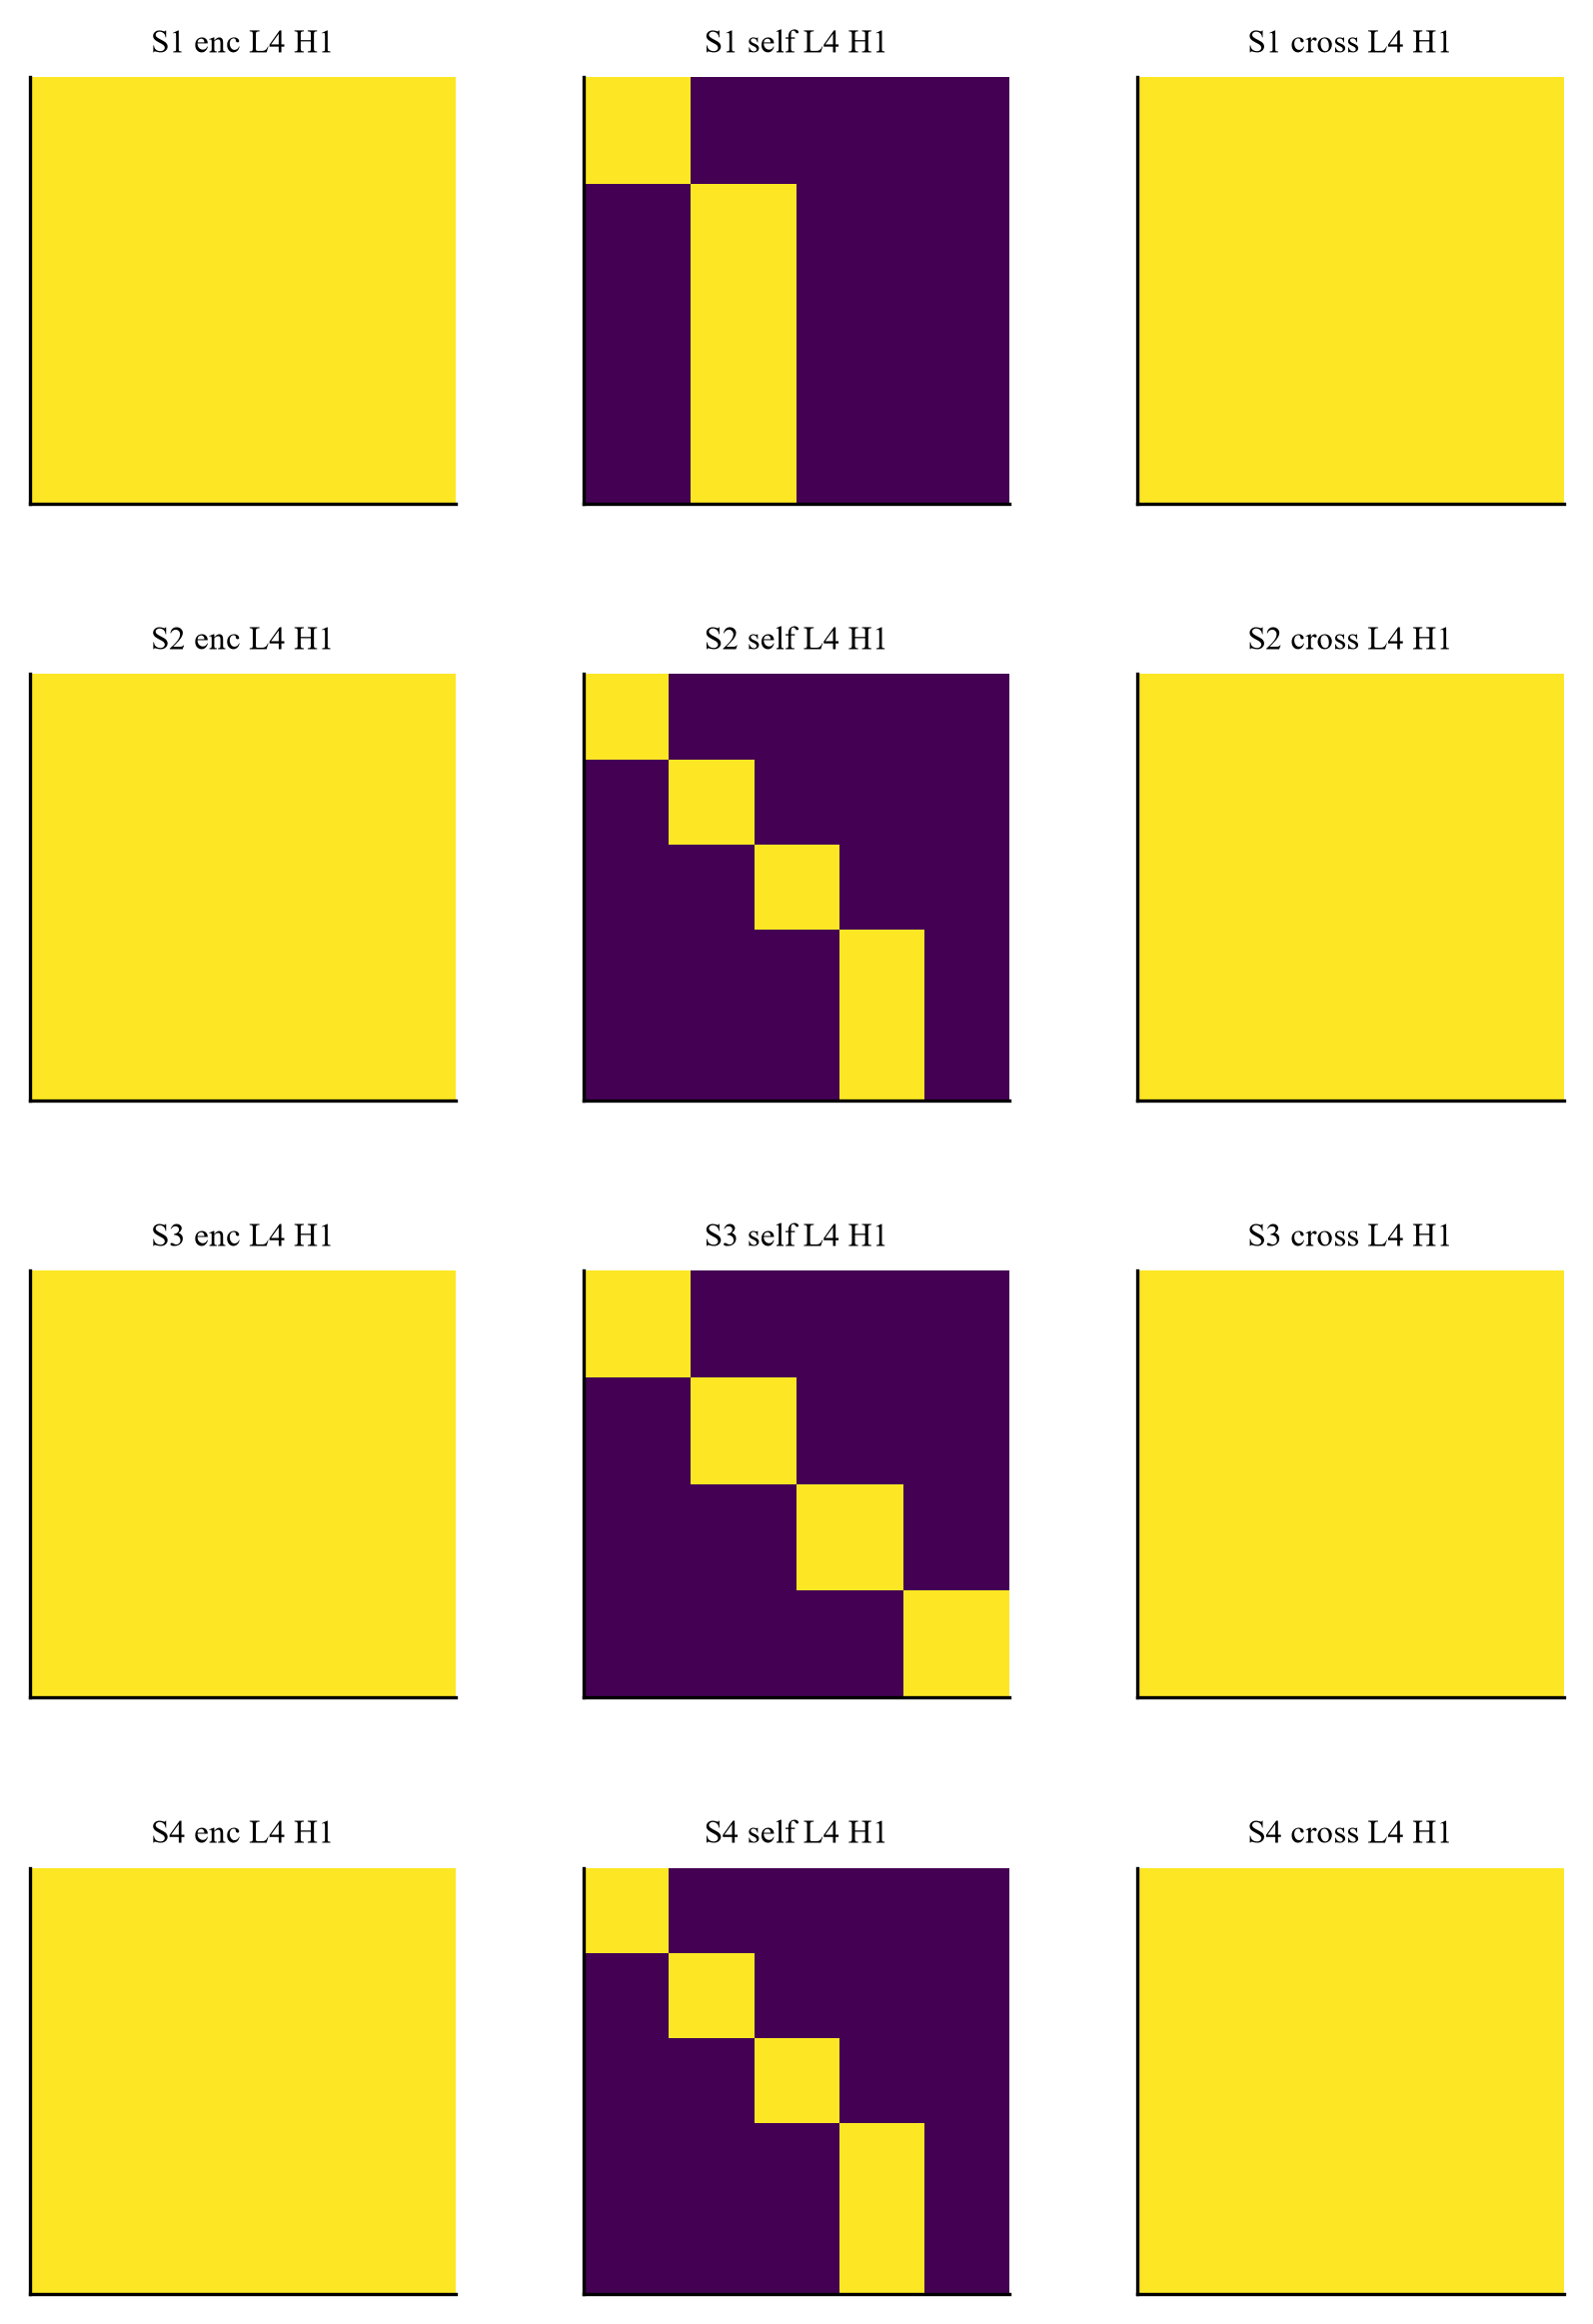
\includegraphics[width=\linewidth]{../figures/per_head/attn_grid_layer4_head1.png}
\caption{Per-head attention for head 1 (0-indexed) across the four test sentences; columns are encoder self / decoder self / decoder cross-attention. Generated via \texttt{python visualize\_attention.py -{-}per-head -{-}head 0 -{-}num-sentences 4 -{-}layer -1}.}
\label{fig:attn-per-head}
\end{figure}

\textit{La Figura~\ref{fig:attn-per-head} examina la cabeza 1 (índice base cero) del último nivel sobre las oraciones de prueba de seis tokens de contenido seleccionadas mediante el filtro \texttt{-{}-min-len}, una longitud suficiente para que cada cabeza exhiba un comportamiento diferenciado, en contraste con las secuencias de uno o dos tokens del análisis previo. En el codificador, la cabeza 1 presenta una estructura aproximadamente diagonal con un sesgo moderado hacia el primer token de la secuencia ---el patrón de \textit{attention sink} descrito por Xiao et al. (2024) para entradas breves. Este predominio del ancla inicial coexiste con asignaciones débiles pero observables fuera de la diagonal, en particular hacia los tokens finales, lo que sugiere que la cabeza comienza a distribuir atención más allá del primer token de la oración. En el decodificador, la auto-atención preserva estrictamente la estructura triangular inferior impuesta por la máscara causal, lo que constituye una verificación adicional de la corrección de la implementación. La atención cruzada, por el contrario, permanece mayormente difusa: la cabeza 1 distribuye la masa de probabilidad entre los tokens fuente sin decantarse de manera concluyente por ninguno de ellos, síntoma coherente con el régimen de sub-entrenamiento descrito en la Sección~5.3 y con la brecha persistente entre la perplexity de validación del modelo word-level (149.84) y la alcanzada por la línea base con BPE (12.39). En conjunto, la cabeza 1 no manifiesta todavía la especialización nítida (\textit{previous-token head}, cabeza \textit{null}, atención focalizada a un token fuente específico) que caracteriza a los Transformers plenamente entrenados; empero, la mayor complejidad sintáctica de las oraciones elegidas elimina el sesgo introducido por secuencias extremadamente cortas y deja preparado el terreno para reproducir este análisis sobre el modelo hand-rolled entrenado con BPE, una vez que concluya la corrida correspondiente en Colab.}
